\documentclass[licencjacka]{pracamgr}
\usepackage{polski}
\usepackage[utf8]{inputenc}
\usepackage[table]{xcolor}
\usepackage{array}
\usepackage{amssymb}
\usepackage{amsmath}
\usepackage{amsthm}
\usepackage[pdftex]{graphicx}
\usepackage{underscore}
\usepackage{hyperref}
\usepackage{caption}
\usepackage{xcolor}
\usepackage{color}
\usepackage{listings}
\lstset{ %
  language=R,                     % the language of the code
  basicstyle=\footnotesize,       % the size of the fonts that are used for the code
  numbers=left,                   % where to put the line-numbers
  numberstyle=\tiny\color{gray},  % the style that is used for the line-numbers
  stepnumber=1,                   % the step between two line-numbers. If it's 1, each line
                                  % will be numbered
  numbersep=5pt,                  % how far the line-numbers are from the code
  backgroundcolor=\color{white},  % choose the background color. You must add \usepackage{color}
  showspaces=false,               % show spaces adding particular underscores
  showstringspaces=false,         % underline spaces within strings
  showtabs=false,                 % show tabs within strings adding particular underscores
  frame=single,                   % adds a frame around the code
  rulecolor=\color{black},        % if not set, the frame-color may be changed on line-breaks within not-black text (e.g. commens (green here))
  tabsize=2,                      % sets default tabsize to 2 spaces
  captionpos=b,                   % sets the caption-position to bottom
  breaklines=true,                % sets automatic line breaking
  breakatwhitespace=false,        % sets if automatic breaks should only happen at whitespace
  title=\lstname,                 % show the filename of files included with \lstinputlisting;
                                  % also try caption instead of title
  keywordstyle=\color{blue},      % keyword style
  commentstyle=\color{dkgreen},   % comment style
  stringstyle=\color{mauve},      % string literal style
  escapeinside={\%*}{*)},         % if you want to add a comment within your code
  morekeywords={*,...}            % if you want to add more keywords to the set
} 

\author{Xxx Yyy}
\nralbumu{000000}
\title{Sugerowanie wyboru ścieżki kształcenia zintegrowane z USOS}
\tytulang{Recomendation of educational path integrated with USOS}
\kierunek{Informatyka}
\opiekun{dra Roberta Dąbrowskiego\\
Pion Zastępcy Kanclerza ds. Informatycznych}
\date{??? 2015}
\dziedzina{
11.0 Matematyka, Informatyka:\\
11.3 Informatyka\\
}
\klasyfikacja{
Information systems\\
Information systems applications\\
Decision support systems\\
Data analytics
}
%\TODO dodać litery/numery wierzchołków w klasyfikacji
\keywords{słowa kluczowe}
%\newtheorem{defi}{Definicja}[section]
\graphicspath{ {./img/} }
\begin{document}
\maketitle
\begin{abstract} ~\\ \indent
Praca poświęcona jest systemowi Hermes, który ma na celu rekomendację przedmiotów dla studentów. Znajduje się w niej opis funkcjonalności, architektury, implementacji, zastosowanych algorytmów oraz organizacji pracy nad projektem.
\end{abstract}
\tableofcontents
\chapter{Wstęp}


 \section{Opis Projektu}


~\\ \indent Głównym celem projektu Hermes było stworzenie serwisu internetowego 
wspierającego studentów w procesie zoptymalizowania wyboru przedmiotów.
Serwis ma za zadanie 
umożliwić studentom lepsze planowanie ścieżki studiów i kariery zawodowej
poprzez proponowanie przedmiotów, które mogą pasować do ich upodobań i predyspozycji. 

Dodatkowym spełnionym wymaganiem projektu jest oferowanie usług przewidywania dla konkretnych studentów ocen z przedmiotów, których jescze nie ukończyli lub bądź nie podjęli.

Serwis oferuje również wsparcie dla uniwersytetu w postaci
przewidywania ilości studentów którzy zapiszą się na konkretny przedmiot. \\
\indent W celu obliczania predykcji system wykorzystywać będzie uczenie maszynowe na statystykach wszystkich studentów Uniwersytetu, a także ewentualnie wybrane przedmioty i uzyskane oceny przez studenta proszącego o propozycję. \\ \\
\indent Projekt został zrealizowany na zlecenie działu sieci komputerowych Uniwersytetu Warszawskiego.
\newpage
\section{od Autorów}

~\\ \indent Wybraliśmy ten projekt, ponieważ sami jesteśmy studentami i jesteśmy świadomi trudności związanych z wyborem przedmiotów. Oferta programowa Uniwersytetu Warszawskiego jest ogromna. W chwili pisania tej pracy po wyszukaniu w systemie usos zwróconych jest ponad 20000 przedmiotów! Dodatkowo opisy często są niejasne, szczątkowe, bądź brakuje syllabusu. Czasem tematyka przedmiotu obieralnego jest na tyle odmienna od dotychczasowego materiału poznanego przez studenta, że może on nie być świadomym, czy dany materiał odpowiada jego predyspozycjom i preferencjom.
\\ \indent Pragniemy zaadresować te problemy za pomocą systemu Hermes. Pisząc go, przyświecała nam idea stworzenia drogowskazu dla studentów, którzy nie są pewni, w jakim kierunku powinni się specjalizować. Wierzymy, iż system dzięki udanym sugestiom zwiększy liczbę studentów, którzy będą naprawdę zainteresowani tematyką przedmiotu, a zmniejszy liczbę studentów zapisanych na przedmioty zupełnie niedopasowane do ich predyspozycji, co często kończy się słabą oceną bądź nawet brakiem zaliczenia. Dzięki temu skorzystają na tym studenci, którzy z większym prawdopodobieństwem zapiszą się na pasujące do ich osiągnięć i predyspozycji przedmioty, z których zdobędą możliwie wiele interesującej ich wiedzy. Zmniejszy się również dla nich ryzyko zapisania się na przedmiot, który w ogóle nie pasuje do ich zainteresowań. Zyska również Uniwersytet, którego studenci będą bardziej zadowoleni z oferty programowej, wzrośnie jakość wiedzy absolwentów oraz lepiej zostanie wykorzystany potencjał studentów. Pomoże to uczelnii być lepiej postrzeganą, bardziej pożądaną przez przyszłych studentów a także zwiększć jej prestiż.
\\ 
\begin{flushright}
Tomasz Grabowski \\
Adam Markiewicz \\
Albert Rozmus \\
Krzysztof Rutkowski \\
Wiktor Zuba 
\end{flushright}

\chapter{Funkcjonalności}
~\\ \indent
Przy wejciu na stronę systemu użytkownik zostaje poproszony o wybranie opcji logowania: "Logowanie dla Studentów" bądź "Logowanie dla Pracowników". \\ \par
~\\
\begin{minipage}{\linewidth}
	 \centering
           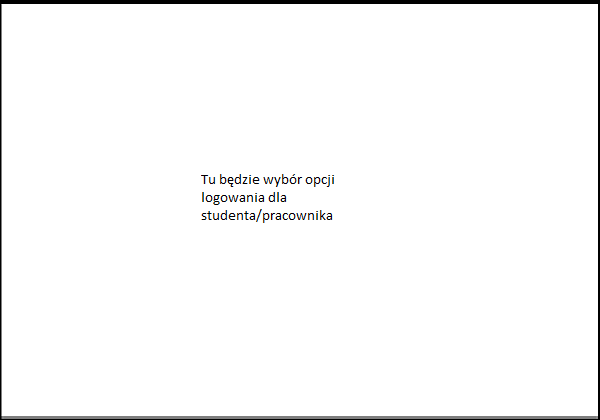
\includegraphics[scale=0.7]{loginlic.png}
	\text{Ekran wyboru opcji logowania}
\end{minipage} \\ \\ \\

 Poniższe podrozdziały opisują funkcjonalności zależne od wybranej opcji.

\section{Funkcjonalności dla Studentów}
~\\ \indent
W tym podrozdziale znajduje się opis funkcjonalności dostępnych dla użytkownika po wybraniu przy logowaniu do systemu opcji "Logowanie dla Studentów". Najpierw student proszony jest o logowanie. \par
~\\
\begin{minipage}{\linewidth}
	 \centering
           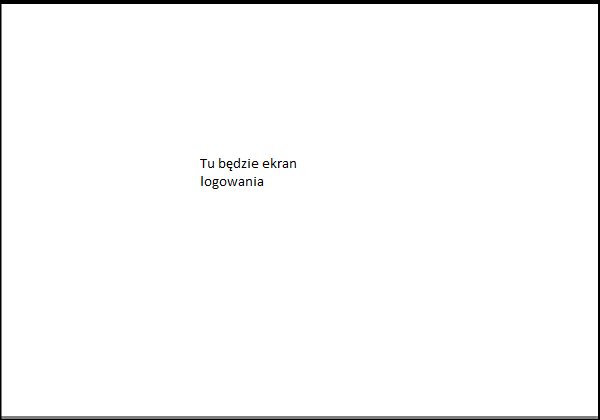
\includegraphics[scale=0.7]{logowanielic.png}
	\text{Ekran logowania dla studentów}
\end{minipage} \\

W przypadku udanej autoryzacji pojawia się interfejs użytkownika który umożliwia wybór między trzeba opcjami : predykcją ocen, rekomendacją seminariów oraz rekomendacją przedmiotów. \par
~\\
\begin{minipage}{\linewidth}
	\centering
           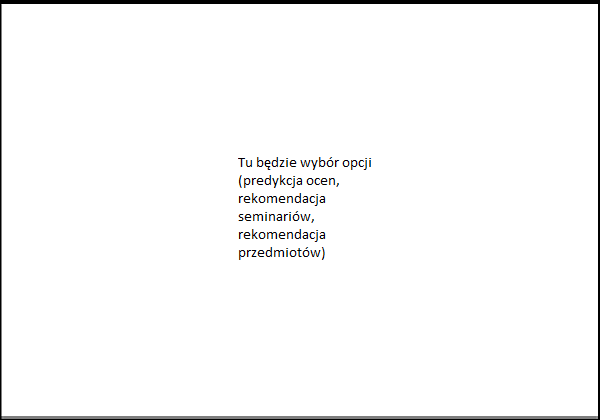
\includegraphics[scale=0.7]{wyborstudent.png}
	\text{Interfejs użytkownika-studenta z wyborem typu predykcji}
\end{minipage} \\ 



\subsection{Predykcja ocen}
~\\ \indent
Po wybraniu opcji predykcji ocen student otrzymuje nowy interfejs.  \par
~\\
\begin{minipage}{\linewidth}
	\centering
           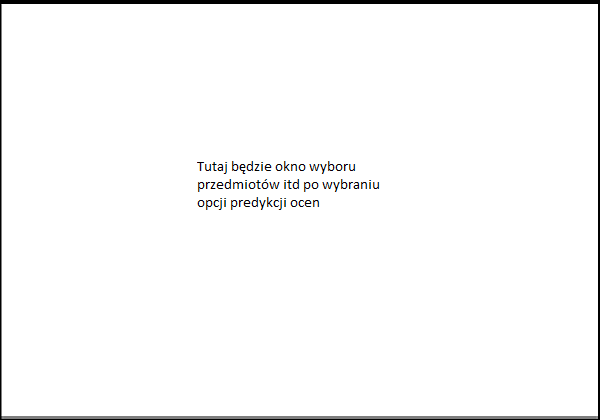
\includegraphics[scale=0.7]{predykcjaocenstart.png}
	\text{Interfejs dla trybu predykcji oceny z przedmiotu}
\end{minipage} \\ \\


Wybiera w nim z odpowiedniego menu przedmiot z którego oczekuje predykcji i prosi o zwrócenie wyniku. System na podstawie danych studenta pobranych za pomocą USOS API przy logowaniu dokonuje odpowiednich obliczeńi i zwraca predykcję studentowi w widocznym polu zatytułowanym "Przewidywana ocena". \\ \par 
 ~\\
\begin{minipage}{\linewidth}
	\centering
           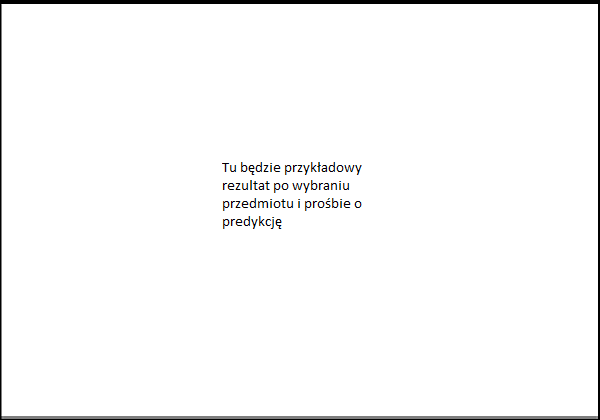
\includegraphics[scale=0.7]{predykcjaocenresult.png}
	\text{Przykładowy rezultat zapytania o predykcję oceny}
\end{minipage} \\ 

\subsection{Remomendacja seminariów}
~\\ \indent
Po wybraniu opcji rekomendacji seminariów student staje przed wyborem dwóch opcji : wybierz najlepsze bądź pokaż ranking. \par 
~\\
\begin{minipage}{\linewidth}
	\centering
           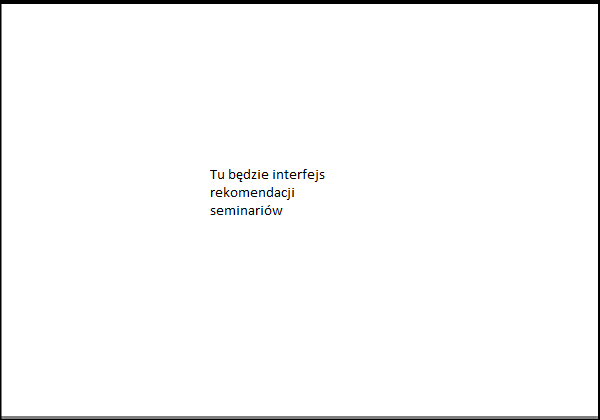
\includegraphics[scale=0.7]{reksem.png}
	\text{Interfejs rekomendacji seminariów}
\end{minipage} \\ 

W obu wypadkach system korzysta z pobranego za pomocą USOSApi programu studiów studenta. Jeżeli student ma więcej niż 1 aktywny kierunek studiow, system prosi go o wybór programu, dla którego predykcja seminariów go interesuje. W zależności od wybranej opcji student otrzymuje jedno seminarium które wg systemu najbardziej pasuje do studenta badź też ranking seminariów od najbardziej pasującego do najmniej wg predykcji systemu. \par
~\\
\begin{minipage}{\linewidth}
	\centering
           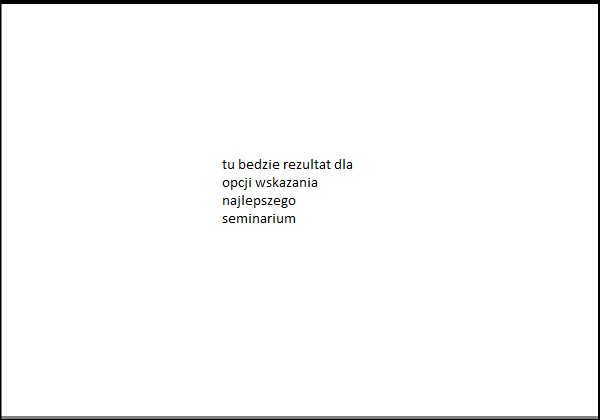
\includegraphics[scale=0.7]{bestsem.png}
	\text{Przykładowy rezultat prośby zarkeomendowanie najlepszego seminarium}
\end{minipage} \\  
~\\
\begin{minipage}{\linewidth}
	\centering
           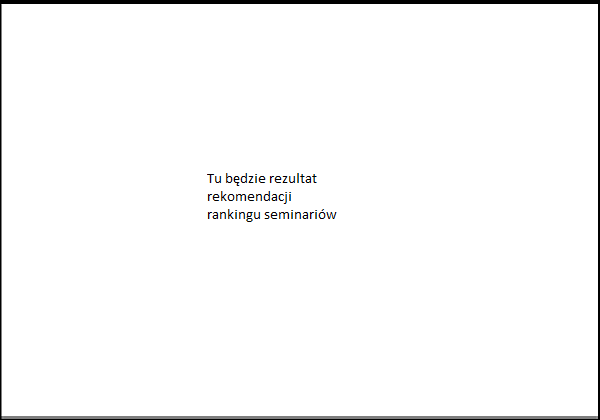
\includegraphics[scale=0.7]{ranksem.png}
	\text{Przykładowy rezultat prośby o obliczenie rankingu seminariów}
\end{minipage} \\ 


\subsection{Rekomendacja przedmiotów} ~\\ \indent
Po wybraniu opcji rekomendacji przedmiotów student otrzymuje wybór kilku opcji. Może wybrać opcje "dobierz przedmioty do seminarium", "dobierz przedmioty do zainteresowań" bądź "znajdź najłatwiejsze". \par
 ~\\
\begin{minipage}{\linewidth}
	\centering
           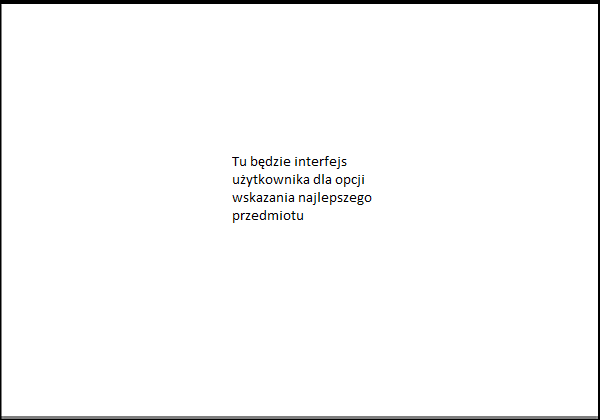
\includegraphics[scale=0.7]{bestprzed.png}
	\text{Interfejs użytkownika dla opcji rekomendacji przedmiotów}
\end{minipage} \\  \\ \\
\indent W przypadku wyboru pierwszej z nich, student jest proszony o wybór interesującego go seminarium. Na tej podstawie system zwraca listę 5 przedmiotów których student nie zdawał, które są wg systemu najbardziej powiązane z wybranym seminarium. \par
 ~\\
\begin{minipage}{\linewidth}
	\centering
           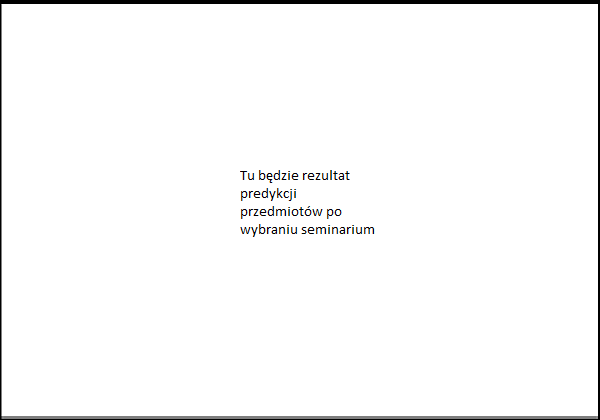
\includegraphics[scale=0.7]{bestprzedsem.png}
	\text{Przykładowy rezultat dla rekomendacji przedmiotów do seminarium}
\end{minipage} \\ 


W przypadku wyboru drugiej opcji, student otrzymuje listę 5 przedmiotów powiązanych z jego programem studiów, które najbardziej do niego pasują na podstawie zaliczanych przez niego przedmiotów i wyników z nich otrzymanych. \par
 ~\\
\begin{minipage}{\linewidth} 
	\centering
           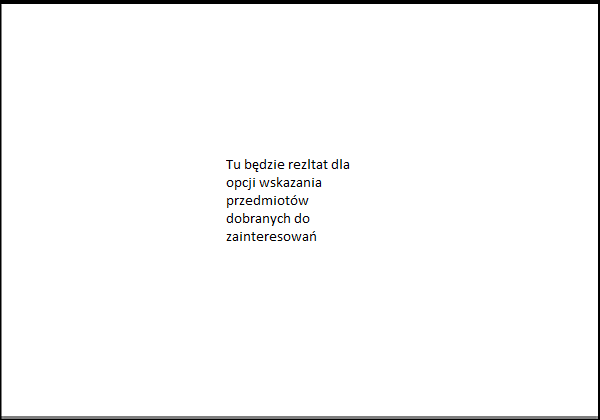
\includegraphics[scale=0.7]{bestprzedzainteresowania.png}
	\text{Przykładowy rezultat dla rekomendacji przedmiotów wg zainteresowań studenta}
\end{minipage} \\ 

 W przypadku wyboru trzeciej opcji, system zwraca 5 przedmiotów powiązanych z programem studiów, które według predykcji student ma największą szansę zdać na dobrą ocenę. \par
 ~\\
\begin{minipage}{\linewidth}
	\centering
           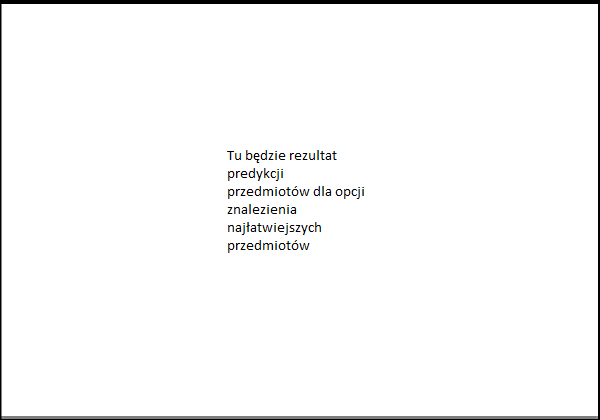
\includegraphics[scale=0.7]{bestprzedeasy.png}
	\text{Przykładowy rezultat dla rekomendacji przedmiotów wg zainteresowań studenta}
\end{minipage} \\ 
\section{Funkcjonalności dla Administracji}
~\\ \indent
Poniższy podrozdział opisuje funkcjonalność dostępną po zalogowaniu przez opcję "Logowanie dla Pracowników", dostępnej po udanej autoryzacji przed odpowiedni formularz. \par
 ~\\
\begin{minipage}{\linewidth}
	\centering
           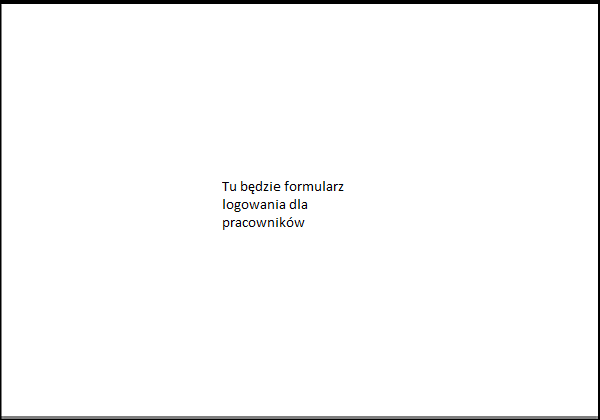
\includegraphics[scale=0.7]{logowanieprac.png}
	\text{Formularz logowania dla pracowników}
\end{minipage} \\ 

\subsection{Predykcja popularności przedmiotów} ~\\ \indent
Po wybraniu opcji przewidywania popularności przedmiotów pracownik z menu może wybrać przedmiot, a następnie osobę prowadzącą i semestr akademicki. \par
 ~\\
\begin{minipage}{\linewidth}
	\centering
           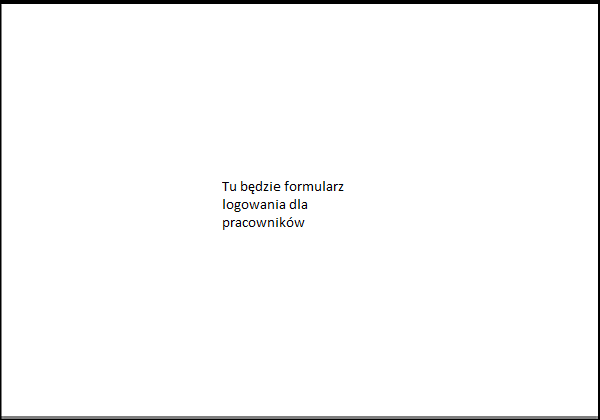
\includegraphics[scale=0.7]{logowanieprac.png}
	\text{Interfejs dla predykcji popularności przedmiotów}
\end{minipage} \\ \\ \\
\indent Na podstawie tych danych system zwraca przewidywaną liczbę osób zapisanych na przedmiot w polu zatytułowanym "przewidywana liczba uczestników". \par
 ~\\
\begin{minipage}{\linewidth}
	\centering
           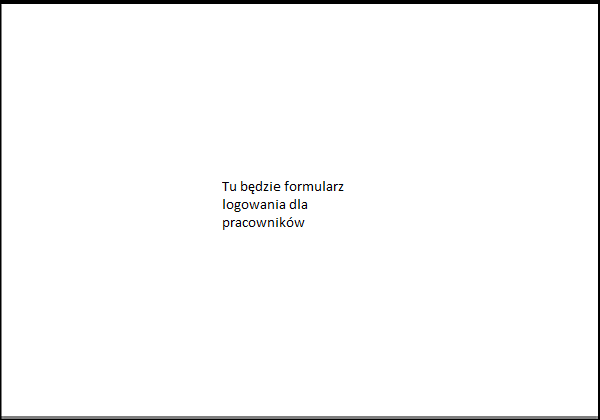
\includegraphics[scale=0.7]{logowanieprac.png}
	\text{Przykładowy rezultat dla predykcji popularności przedmiotów}
\end{minipage} \\ 
 

 \chapter{Architektura} 
\section{Schemat Architektury}
~\\
\begin{minipage}{\linewidth} 
	\centering
           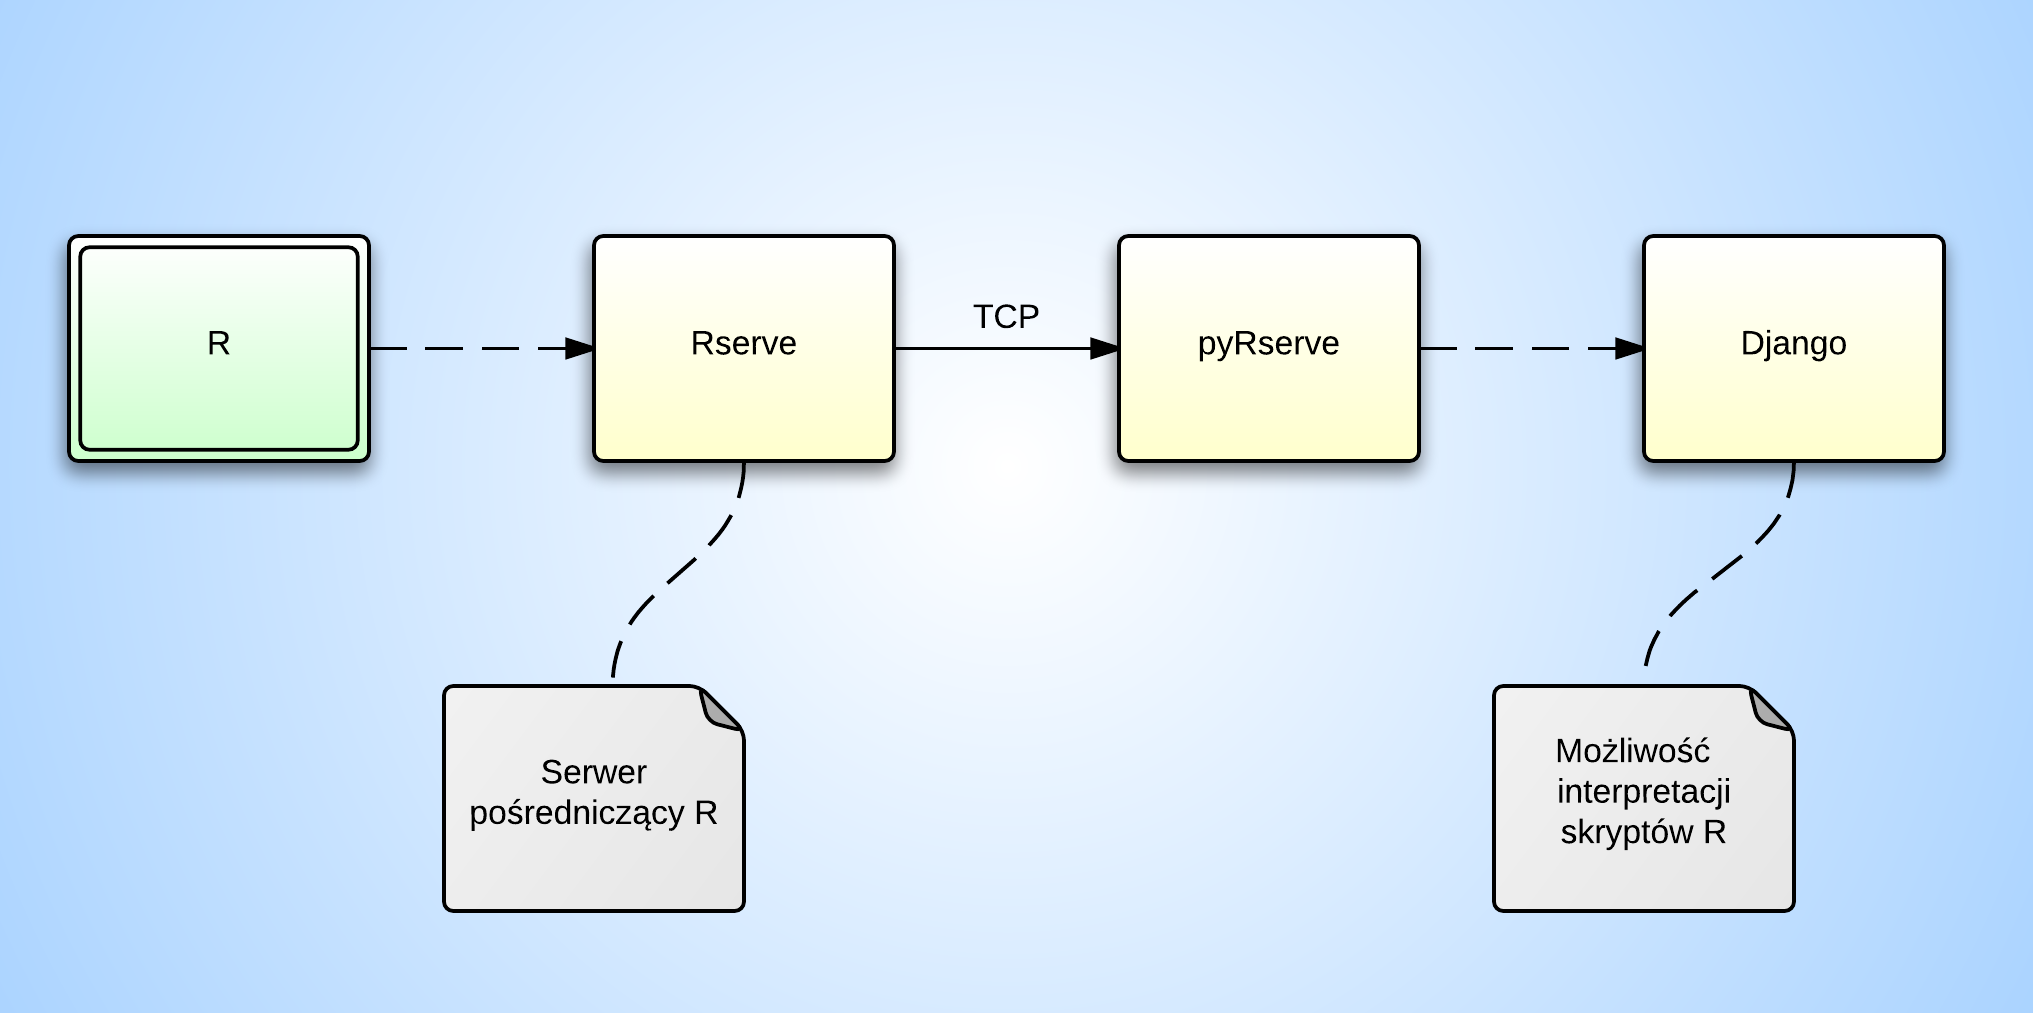
\includegraphics{architekturaR.png}
	\text{Architektura systemu Hermes}
\end{minipage} \\ \\ \\
 W architekturze i logice naszego systemu wyróżniamy następujące komponenty:
 \begin{itemize}
 
\item \textbf{Chmura} - Sercem systemu jest główny serwer wraz z innymi usługami znajdujący się w chmurze internetowej. Znajduje się na niej serwer bazy danych, serwer WWW oraz serwer usług analitycznych.

\item \textbf {RDB} - Relacyjna baza danych zawierająca statystyczne dane dotyczące zdawalności przedmiotów przez studentów, ich zapełnienia, popularność itd. Stanowi bazę do tworzenia predykcji. Zawiera również bazę wyliczonych przez algorytmy rezultatów które wspierają modyfikacj

\item \textbf{Serwer analityczny} - serwer na którym odbywa się preprocessing, przetwarzanie danych oraz obliczanie predykcji dla studenta.

\item \textbf{Moduł integracyjny} - moduł który łączy się z bazą danych systemu USOS i konwertuje przekazywane z niej dane na format bazy danych systemu Hermes
 
\item \textbf{USOS Api} - API udostępniane przez system USOS. Nasz system wykorzystuje je w celu zebrania danych zalogowanego użytkownika niezbędnych do zarekomendowania mu tego czego oczekuje.

\item \textbf{Strona WWW} - interfejs za pomocą którego użytkownik może przesyłać prośby o wykonanie udostępnianych przez system rekomendacji.

\item \textbf{Serwer WWW} - udostępnia użytkownikom stronę internetową, w naszym systemie pośredniczy między interfejsem użytkownika a bazą danych. Pośredniczy również w komunikacji z serwerem analitycznym.

  
\end{itemize}

\section{Schemat współdziałania komponentów architektury}
~\\ \indent
Schemat działania i komunikacji między poszczególnymi komponentami wygląda następująco:
\begin{enumerate}

\item Na samym początku działania system tworzy relacyjną bazę danych zawierającą dane statystyczne z USOSa. Przy pobieraniu danych z USOS wykorzystywany jest moduł integracyjny w celu dostosowania danych.

\item Serwer analityczny dokonuje obliczeń i wstępnego przetworzenia zebranych danych aby usprawnić wyliczanie przyszłych predykcji.

\item Po wykonaniu przetworzenia danych i obliczenia statystyk aktywuje się serwer WWW i system staje się dostępny dla użytkowników.

\item Użytkownik wchodzi na stronę i otrzymuje formularz logowania. W przypadku udanego logowania serwer pobiera dane użytkownika za pośrednictwem USOS Api i zwraca stronę WWW - interfejs użytkownika.

\item Serwer WWW po odebraniu prośby o rekomendacje przesyła żądanie do serwera analitycznego z poleceniem obliczenia predykcji, Wykorzystuje się przy tym odebrane wcześniej dane użytkownika.

\item Serwer WWW odbiera rezultat zapytania od serwera analitycznego i wyświetla go użytkownikowi za pośrednictwem strony WWW.

\end{enumerate}


 \chapter{Technologia}
Technologie wykorzystywane w naszym systemie: \par

 \begin{minipage}{\linewidth}
            \centering
            
\includegraphics[width=10cm, height = 3cm]{azure.jpg}
\end{minipage} \\ \\
\noindent 
 \textbf{Microsoft Azure} - Azure jest komercyjną platformą obsługiwaną przez Microsoft. Udostępnia ona usługi związane z chmurą internetową (tzw cloud-computing). W naszym systemie znajduje sie na niej serwer WWW a także serwer bazy danych. \par ~\\
\begin{minipage}{\linewidth}
            \centering
            
\includegraphics[width=10cm, height = 3cm]{sql-server-2014-logo.png}
\end{minipage} \\ \\

\noindent \textbf{Microsoft SQL Server 2014} - Komercyjny serwer bazodanowy udostępniany przez Microsoft. Znajduje się w nim relacyjna baza danych zawierająca dane niezbędne do stworzenia modelu analitycznego.  \par ~\\

\begin{minipage}{\linewidth}
            \centering
            
\includegraphics[width=4cm, height = 4cm]{R.png}
\end{minipage} \\ \\

\textbf{R} - język skryptowy używany w celu analizy danych a także obliczania predykcji dla studentów bądź uniwersytetu. \par
\begin{itemize}

\begin{figure}
\centering
\begin{minipage}{0.45\textwidth}
\centering

\includegraphics[width=6cm, height = 3cm]{python-logo-master-v3-TM.png}
\end{minipage}\hfill
\begin{minipage}{0.45\textwidth}
\centering

\includegraphics[width=6cm, height = 3cm]{django-logo-negative.png}
\end{minipage}
\end{figure}

\item \textbf{Python oraz Django} - technologie, za pomocą których tworzymy webowy interfejs użytkownika. \par ~\\

\begin{minipage}{\linewidth}
            \centering
            
\includegraphics[width=7cm, height = 2.5cm]{usosapi.jpg}
\end{minipage} \\ \\

\item \textbf {USOS Api} - API udostępniane przez system USOS. Nasz system wykorzystuje go w celu zebrania danych zalogowanego użytkownika
niezbędnych do rekomendacji.

\end{itemize}

\chapter{Zastosowane Algorytmy}
~\\ \indent Przy tworzeniu algorytmow wykorzystalismy pakiet statystyczny R. Gwarantowal on duza kontrole nad algorytmami,
ktorych uzywalismy. W naszej pracy pojawily sie wszystkie najwazniejsze rodzaje algorytmow uzwanych w eksploracji danych:
\begin{itemize}
 \item klasyfikacja
 \item poszukiwanie regul asocjacyjnych
 \item grupowanie
\end{itemize}
Najwiecej pojawilo sie zastosowan pierwszej z metod. Czasem uzywalismy tez podejscia statystycznego, nie uczac jakiegos modelu,
lecz podejmujac decyzje na podstawie statystyk. W zastosowanych algorytmach czesto uzywalismy odpowiednio zdefiniowanej
funkcji odleglosci miedzy obiektami w naszym modelu. Obiektem byl tu wektor $n$-elementowy ocen studenta pomnozonych o 2 oraz 11
w przypadku oceny $5!$ a takze $0$, gdy student nie uczestniczyl w przedmiocie, dla dwoch takich wektorow definiujemy miare 
odleglosci miedzy studentami $v=(v_{1},..,v_{n})$ i $w=(w_{1},..,w_{n})$:
\[
 dist(v,w) = \sum_{k=1}^n \begin{cases} 10 &\text{gdy } (v_{k} = 0)\oplus(w_{k} = 0) \\|w_{k}-v_{k}| &\text{wpp}  \end{cases}
\]
kod w R:
\lstinputlisting{dist.R}
Podana funkcja mocniej wyraza fakt, ze studenci brali rozne przedmioty niz to ze mieli rozne oceny. Uzywalismy
jej w algorytmach opartych na metodzie k najblizszych sasiadow, ktorej uzywalismy w wielu predykcjach. W naszym systemie 
mielismy kilka rodzajow predykcji i rekomendacji:
\begin{itemize}
 \item proponowanie przedmiotow
 \item predykcja seminarium
 \item predykcja ocen
\end{itemize}
\subsection{Algorytmy uzyte przy proponowaniu przedmiotow}
Przy proponowaniu przedmiotow obieralnych uzylismy 4 strategii:
\begin{itemize}
 \item wyliczanie regul asocjacyjnych
 \item strategia najblizszych sasiadow
 \item przydzial w oparciu o statystyki
 \item przydzial losowy
\end{itemize}
Reguly asocjacyjne wyliczylismy za pomoca algorytmu apriori dostepnego w pakiecie 'arules'. Algorytm bral na wejsciu koszyki
przedmiotow, czyli zestawy przedmiotow obieralnych, ktore wzieli poszczegolni studenci, zas na wyjsciu zwracal reguly postaci
'jesli student wzial przedmioty $p_{1},..,p_{k}$ to prawdopodobnie wezmie tez przedmiot $p_{l}$'. To 'prawdopodobnie' 
zalezy od miar $support$ i $confidence$ podawanych na wejsciu algorytmu.
Miary $support$ i $confidence$ ustawilismy tak, by regul nie bylo za duzo, ale tez byly sensowne. \\
Strategia najblizszych sasiadow zostala uzyta w oparciu o miare $dist$ przedstawiona wyzej. Polegala ona na tym, ze 
sposrod pewnej liczby najblizszych studentowi, ktoremu chcemy cos zaproponowac, sasiadow, bierzemy przedmioty, ktore oni brali.
W tym podejsciu probujemy zaklasyfikowac studenta do podobnej grupy i przydzielic mu to co brali 'podobni' studenci. Kod w R:
\lstinputlisting{nearestSub.R}
Przydzial w oparciu o statystyki to propozycja przedmiotow, ktore prawdopodobnie byloby studentowi najlatwiej zaliczyc.
Statystyke 'latwosci' przedmiotu stanowila srednia wazona supportu, sredniej ocen i zdawalnosci przedmiotu. \\
Przydzial losowy polegal na braniu z jenostajnym rozkladem prawdopodobieństwa przedmiotow, ktorych student jeszcze nie wzial.
\subsection{Algorytmy uzywane przy predykcji seminariow}
Przy proponowaniu seminariow uzylismy 2 strategii:
\begin{itemize}
 \item klasyfikator najblizszych sasiadow
 \item klasyfikator lasow losowych
\end{itemize}
Klasyfikator najblizszych sasiadow, tak jak w przypadku proponowania przedmiotow, rowniez korzystal ze zdefniowanej funkcji
odleglosci i ze zbioru decyzji dla najblizszych sasiadow, czyli seminarium, ktore wybrali najblizsi sasiedzi, jako proponowane
wybieral mode, czyli najczesciej wystepujace wsrod sasiadow seminarium. \\
Klasyfikator lasow losowych budowalismy w oparciu o pakiet 'randomForest'. Jest to klasyfikator, ktory buduje sie w oparciu o
klasyfikacje na pewnej liczbie drzew decyzyjnych, nastepnie agregujac decyzje z tych drzew, najczesniej przez glosowanie.
Dawal on gorsze wyniki niz klasyfikator najblizszych sasiadow.
Na danych testowych,skutecznosc klasyfikatora knn wynosila $0.45$ podczas gdy skutecznosc lasow losowych tylko $0.26$. Jednak
zaleta tego klasyfikatora jest to, ze buduje on juz wczesniej model i decyzja dla danych wejsciowych studenta obliczana
jest bardzo szybko, w przeciwienstwie do klasyfikatora knn. Kod w R:
\lstinputlisting{rf.R}
\subsection{Algorytmy uzywane przy predykcji ocen}
TODO

\chapter{Organizacja pracy oraz podział obowiązków} ~\\

\section{Praca nad systemem} ~\\

Za namową zamawiającego na początku zdecydowaliśmy się zrealizować projekt za pomocą technologii koncernu Microsoft. Otrzymaliśmy od niego licencję Bizspark która dała nam licencję na swobodne wykorzystywanie produktów Microsoftu przez 2 lata. Dodatkowo Bizspark umożliwiał korzystanie z usługi Azure w zakresie abonamentu w wysokości 150 euro na miesiąc. Dlategoywybraliśmy chmurę Azure jako nasz serwer. Planowaliśmy dodatkowo zrealizować obliczanie predykcji za pomocą Sql Server Analysis Services a frontend za pomocą .NET. \\

Z projektem jednak wiązały się dość znaczące problemy. Pierwszym z nich była zmiana technologii użytej w celu obliczania predykcji, na którą zdecydowaliśmy się w lutym. Przed rozpoczęciem pracy nad projektem nikt z nas nie znał możliwości Sql Server Analysis Services (SSAS) ani nie tworzył strony internetowej w .NET. O ile z .NET nie było znaczących problemów, usługi analityczne Sql Servera stanowiły dla nas barierę nie do przejścia. Ze względu na dość kiepsko udomkumentowną technologię SSAS, brak szkoleń z tej technologii oraz brak zajęć na uniwersytecie jej poświęconym oraz małej elastyczności algorytmów tej usługi podjęliśmy decyzję o rezygnacji z tego narzędzia. Zdecydowaliśmy się na wykorzystanie języka skryptowego R, z którym dobrze zaznajomione były 2 osoby w zespole. Zmieniliśmy także realizację frontendu z .NET na Django ponieważ główny powód wyboru .NET - pluginy dedykowane dla SSAS, przestał być ważny dla projektu. Z Django obeznane były wszystkie osoby w zespole, a dodatkowym atutem tego wyboru był jeden członek zaspołu posiadającz doświadczenie zawodowe w pisaniu aplikacji w Pythonie. \\

Kolejnym znaczącym problemem była mocno utrudniona praca związana z analizą danych i dobieraniem optymalnych algorytmów. Zamawiający obiecał nam dostarczenie zaszumionych danych z systemu USOS. Czekaliśmy na nie, ponieważ trudno było samemu wymyślić i wygenerować nietrywialne korelacje, zbliżone do rzeczywistości. Próbka takich danych mocno pomogłaby nam z doborem algorytmów predykcyjnych. Jednak zaszumienie okazało się w praktyce niemożliwe a "zwykłych" danych nie mogliśmy otrzymać z powodu ustawy o ochronie danych osobowych. O tych ograniczeniach praktycznie dowiedzieliśmy się dopiero w kwietniu, co mocno nam popsuło pracę nad algorytmami predykcyjnymi i analizą ich jakości która niestety nie została wykonana na danych produkcyjnych.

\section{Organizacja Pracy} ~\\


Naszym repozytorium był git. Drzewo projektu w repozytorium prezentuje się następująco:

TODO : tu będzie drzewko naszego repo.

Przydział zadań do osób i planowanie pracy zostały zrealizowane za pomocą portalu Redmine. \\

Praca na początku projektu przebiegała dość chaotycznie, z długimi przerwami. Dużą blokadą były dla nas problem z efektywną pracą nad predykcjami z SSAS oraz brak danych bliższych rzeczywistości utrudniający nam wyjście poza teoretyczne rozważanie o algorytmach. Realną pracę wychodzącą poza studiowanie dokumentacji i metodę prób i błędów prowadząca do nikąd zaczęliśmy dopiero po decyzji o zmianie technologii w lutym. Praca odbywała się wtedy w cotygodniowych iteracjach, a znacząco przyśpieszyła w kwietniu po ostatecznej decyzji o braku możliwości otrzymania jakichkolwiek danych przypominających rzeczywiste. Niestety ze względu na niezbyt długi pozostały wówczas czas nie udało nam się zrealizować wszystkich planów.

\section{Podział Obowiązków} ~\\

TODO (przy działającym serwisie rzetelnie opiszę wkład osób)
~\\ \indent W projekcie Hermes podział pracy był następujący:

\begin{itemize}
\item \textbf{Tomasz Grabowski} - Redakcja licencjatu, prezentacja, pomoc przy tworzeniu danych testowych do bazy.
\item \textbf{Adam Markiewicz} - Administrowanie serwerem umieszczonym na Azure.
\item \textbf{Albert Rozmus} - Pomoc przy tworzeniu frontendu i serwera WWW
\item \textbf{Krzysztof Rutkowski} - Tworzenie frontendu, zarządzanie serwerem analitycznym, pomoc przy tworzeniu modułów dla serwera analitycznego służących predykcji i rekomendacji.
\item \textbf{Wiktor Zuba} - Tworzenie danych testowych do bazy oraz ich relacyjnego modelu. Tworzene modułów dla serwera analitycznego służących predykcj i rekomendacji.
\end{itemize}

\chapter{Podsumowanie} ~\\ \indent


Projekt napotkał na duże przeszkody w trakcie realizacji. Problemy z zamawiającym, z otrzymaniem sensownych danych testowych oraz z nauką Sql Server Analysis Services a także skutecznym wykorzystaniem jego algorytmów z dość znaczącymi limitacjami mocno wpłynęły na czas spędzony na efektywnej pracy nad projektem. Z ubolewaniem przyznajemy, iż realną pracę przynoszącą progres a nie błądzenie w ślepych zaułkach, książkach i dokumentacjach zaczęliśmy dopiero w marcu.

W celu realizacji projektu i usprawnienia pracy musieliśmy podjąć decyzję o zmianie technologii. Umożliwiło nam to mieć większy wpływ na tworzone algorytmy predykcyjne oraz sposób ich działania. Dużym plusem tej zmiany była możliwośc wykorzystania solidnej znajomośc teorii systemów decyzyjnych oraz jej zastosowania w R przez członków zespołu. Zmiana na Django także była skutkiem lepszej znajomości Pythona przez zespół. Uważamy, iż zmiany okazały się w końcowym rozrachunku pozytywne, ponieważ udało nam się zaimplementować system który zawiera większość planowanych na początku funkcjonalności. Dodatkowo, dzięki zastosowanym technologiom, w miarę łatwe jest rozwijanie systemu. W celu zaimplementowania nowych typów predykcji wystarczy napisać nowy skrypt w R i załączyć go do systemu oraz zintegrować z frontendem.

Problemy przy pracy nad projektem niestety uniemożliwiły spełnienie naszych wszystkich założeń. Zabrakło nam czasu na zaimplementowanie funkcjonalności dla pracowników predykujących popularność wybranych przedmiotów wśród studentow. Z przyczyn niezależnych od nas nie udało nam się również przetestować napisanych przez nas algorytmów na prawdziwych danych, przez co nie mieliśmy możliwości praktycznej weryfikacji predykcji. 

Mamy jednak nadzieję, iż pomimo tych trudności system sprawdzi się na prawdziwych danych i okaże się realną, efektywną pomocą dla studentów.


\begin{thebibliography}{99}
\addcontentsline{toc}{chapter}{Bibliografia}
\bibitem[AZR]{AZR} Microsoft
\textit{dokumentacja techniczna Azure} \\
http://azure.microsoft.com/en-us/documentation/
\bibitem[PTN]{ptn}
Python Software Foundation
\textit{dokumentacja techniczna języka Python} \\
https://docs.python.org/2.7/
\bibitem[DGO]{DGO} Django Software Foundation
\textit{dokumentacja techniczna Django} \\ 
https://docs.djangoproject.com/en/1.8/
\bibitem[R]{R} R Development Core Team
\textit{dokumentacja techniczna języka R} \\
http://cran.r-project.org/manuals.html
\bibitem[RSV]{RSV} Simon Urbanek
\textit{dokumentacja techniczna serwera R - modułu RServe} \\
http://www.rforge.net/Rserve/doc.html
\end{thebibliography}
\end{document}